\documentclass{article}
\usepackage[utf8]{inputenc}
% \usepackage{newunicodechar}
% \newunicodechar{fi}{fi}
% \newunicodechar{ff}{ff}
\usepackage{amsmath}
\usepackage{mathtools}
\usepackage{xcolor}
\usepackage{booktabs}
\usepackage{enumerate}
\usepackage{extarrows} % extra arrows
\usepackage{graphicx}                 % 图形
\usepackage{tikz} % draw graph in latex
\usetikzlibrary{decorations.pathreplacing} % decoration package for tikz
\graphicspath{{figures/}}        % 图片文件路径
\newlength\imagewidth
\newcommand{\myref}[1]{Equation \eqref{#1}}
\setlength\imagewidth{0.45\columnwidth}

% \pagestyle{empty}
% \newlength{\defwidth}
% \textwidth = 17.5cm
% \defwidth  = 15.0cm
% \textheight = 26cm
% \topmargin = -2.0cm
% \oddsidemargin = -0.5cm
% \evensidemargin = 0.25cm
% \parindent 0mm
% \sloppy
% \setlength{\parskip}{2mm plus1mm minus1mm}

\title{Pollution Control 2}
\author{Zhao Chi, Wu Haitao}
\date{\today}


\begin{document}
    \maketitle
\section*{Question}

\begin{figure}[ht]
    \centering
    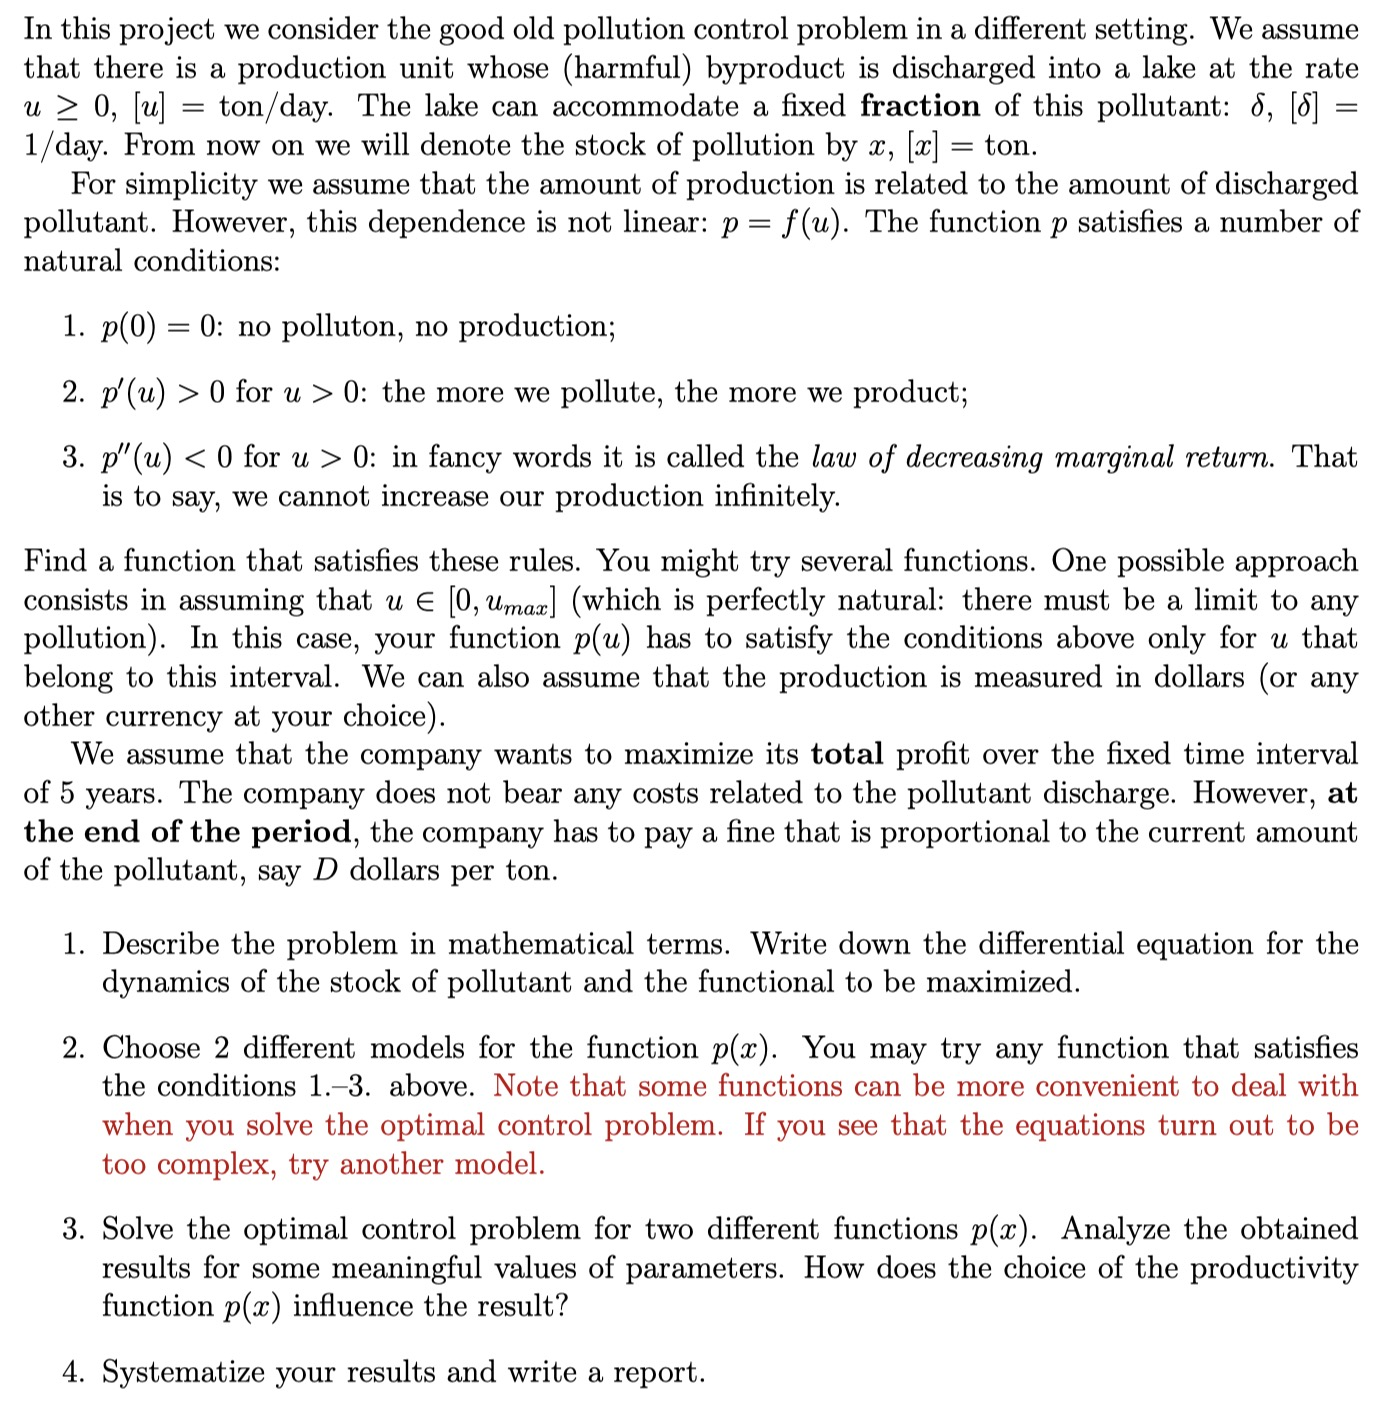
\includegraphics[width=2.2\imagewidth]{Question.png}
    % \caption{Question}
    %   \label{fig:q}
\end{figure}


\section*{Solution}

{\bf Question 1:} Describe the problem in mathematical terms. Write down the differential equation for the dynamics of the pollutant and the functional to be maximized.

From the Question description, it's not hard to find that as the time change, the total amount of pollution increases $u$ per unit time. Besides, consider the absorption of pollutants by the lake itself. Therefore we can write down the relationship in differential equation form.

\begin{equation}\label{cd:initial_condition}
    \dot{x}=u-\delta x, x(0)=x_0 \geq 0
\end{equation}

There are many function $p(u)$ satisfy the following natural conditions:

\begin{enumerate}
    \item $p(0)=0$;
    \item $p'(u)>0\ \text{for}\ u\in(0,u_{max}]$;
    \item $p''(u)<0\ \text{for}\ u\in(0,u_{max}]$.
\end{enumerate}

Before, $p(u)$ is the amount of production, now we assume $p(u)$ is the profit $\text{dollars/unit}$. Indeed do that change doesn't influence our optimal solution. Therefore, the instantaneous payoff function is defined as:

\begin{equation}\label{eq:payoff_funtion_instant}
    f_0(u)=p(u)
\end{equation}

The company want to maximize it's \textbf{total} profit over the fixed time interval of 5 years and the company does not bear any costs related to the pollutant discharge. However, at \textbf{the end of the period}, the company has to pay a fine that is proportional to the current amount of the pollutant, say $D$ dollars per ton. Therefore we have a terminal cost.

\begin{equation}\label{eq:terminal_cost}
    F_0(x(T))=Dx(T)
\end{equation}


Assume \textbf{endpoint} is \textbf{free}, then the total payoff function to be maximized is:

\begin{equation}\label{eq:optfunction_with_terminal_cost}
    J(u,T)=\int_{0}^{T}p(u)dt-Dx(T)\rightarrow \max_{u} 
\end{equation}

\noindent{\bf Question 2:} Choose 2 different models for the function $p(u)$ that satisfies the conditions 1.-3. above.

We need to assure the first order derivative large than $0$, assume $u_{max}=b$. the following two models satisfy conditions 1-3\footnote{For model 2, $p'(u)>0 \text{ for } u>0$ the maximal value occur at the boundary point $b$. But for model 1, $p'(u)>0 \text{ for } u\in(0,b)$ and $p'(b)=0, p''(u)|_{u=b}<0$, the maximal value occur at $u=b$.}. 

\begin{gather}
    \begin{aligned}
        \textbf{Model 1: } & p(u)=-\frac{1}{2}u^2+bu\\
        \textbf{Model 2: } & p(u)=\ln (u+1) 
    \end{aligned}
\end{gather}

\noindent{\bf Question 3:} Solve the optimal control problem for two different functions $p(u)$. Analyze the obtained results for some meaningful values of parameters. How does the choice of the productivity function $p(u)$ influence the results.


{\bf Model 1:} Our optimization problem is:
\begin{equation}
    J(u,T)=\int_{0}^{T}\bigl(-\frac{1}{2}u^2+bu\bigr)dt-Dx(T)\rightarrow \max_{u}\ s.t. \eqref{cd:initial_condition}
\end{equation}
\begin{enumerate}[a)]
    \item Write down the Hamiltonian Function:
            \begin{equation}\label{eq1:hamiltonian}
                H(x,u,\psi)=-\frac{1}{2}u^2+bu+\psi (u-\delta x)
            \end{equation}
    \item It's first order partial derivatives w.r.t $u$ is:
            \begin{equation}
                \frac{\partial }{\partial u}H(x,u,\psi)=-u+b+\psi
            \end{equation}
             According to the first order extreme condition:
             \begin{equation}\label{eq1:optc_with_psi}
                u^*(t)=b+\psi(t)
             \end{equation}
             And $\frac{\partial^2 }{\partial u^2}H(x,u,\psi)\big|_{u=u^*}<0$, we can conclude that the Hamiltonian $H$ is concave w.r.t $u$.
    \item We substituete \eqref{eq1:optc_with_psi} into \eqref{eq1:hamiltonian} to get the maximal Hamiltonian Function:
             \begin{equation}
                \mathcal{H}(x, \psi)=H(x,u^*,\psi)=\frac{1}{2}(b+\psi)^2-\delta\psi x
             \end{equation}
    \item The canonical form is written as:
             \begin{equation}\label{eq1:canonical_form}
                 \begin{dcases}
                    \dot{x}= \frac{\partial }{\partial \psi}H(x,u,\psi)\bigg|_{u=u^*}=b+\psi(t)-\delta x\\
                    \dot{\psi}=-\frac{\partial }{\partial x}H(x,u,\psi)\bigg|_{u=u^*}=\delta\psi(t)
                \end{dcases}
             \end{equation}
    \item From D.E.S \eqref{eq1:canonical_form}, it's not hard to find:
             \begin{equation}\label{eq1:psi_with_psi0}
                 \psi(t)=\psi_0 e^{\delta t}
             \end{equation}
    \item According to D.E.S \eqref{eq1:canonical_form} and Equation \eqref{eq1:psi_with_psi0}, we can find the optimal trajectory:
             \begin{equation}\label{eq1:optx_with_psi0}
                 x^*(t)=x_0e^{-\delta t}+\frac{b}{\delta}(1-e^{-\delta t})+\frac{\psi_0}{2\delta}(e^{\delta t}-e^{-\delta t})
             \end{equation}
    \item There is boundary condition on $\psi$:
    \begin{equation}
        \psi(T)=\psi_0 e^{\delta T}=-\frac{d}{dx}Dx(t)\bigg|_{t=T}=-D
    \end{equation}

    Hence:

    \begin{equation}\label{eq1:psi0}
        \psi_0=-De^{-\delta T}
    \end{equation}

    Then,
    \begin{equation}\label{eq1:psi}
        \psi(t)=-De^{\delta (t-T)}
    \end{equation}

    \item Substitute Equation \eqref{eq1:psi} into Equation \eqref{eq1:optc_with_psi}, we can find the optimal control:
    \begin{equation}
        u^*(t)=b-De^{\delta (t-T)},\ \text{where}\ b\geq D
    \end{equation}

    We need to assure $u^*(t)\geq 0\ \text{for}\ t\in[0,T]$, so condition $b>D$ is necessary.

    \item Substitute Equation \eqref{eq1:psi0} into Equation \eqref{eq1:optx_with_psi0}, we get:
    \begin{equation}\label{eq1:optx}
        x^*(t)=x_0e^{-\delta t}+\frac{b}{\delta}(1-e^{-\delta t})-D\frac{e^{-\delta T}}{2\delta}(e^{\delta t}-e^{-\delta t})
    \end{equation}


    \item  Find the first order derivative w.r.t $t$:
    \begin{equation}\label{eq1:optx_d}
        \frac{dx^*(t)}{dt}=-{\mathrm{e}}^{-\delta \,\left(T+t\right)}\,\left(\frac{D}{2}-b\,{\mathrm{e}}^{T\,\delta }+\frac{D\,{\mathrm{e}}^{2\,\delta \,t}}{2}+\delta \,x_{0}\,{\mathrm{e}}^{T\,\delta }\right)
    \end{equation}

    Under the condition below:

    \begin{equation}\label{conditions:model1}
        \begin{split}
            b\geq D\\
            D-2\,b\,{\mathrm{e}}^{T\,\delta }+2\,\delta \,x_{0}\,{\mathrm{e}}^{T\,\delta }<0\\
            \frac{\sqrt{2\,b\,{\mathrm{e}}^{T\,\delta }-D-2\,\delta \,x_{0}\,{\mathrm{e}}^{T\,\delta }}}{\sqrt{D}}>1\\
            D+2\,\delta \,x_{0}\,{\mathrm{e}}^{T\,\delta }\neq 2\,b\,{\mathrm{e}}^{T\,\delta }\\
            \text{all parameters are large than 0}
        \end{split}
    \end{equation}

    We can find the stationary point:

    \begin{equation}\label{eq1:t^*}
        t^*=\frac{\ln\left(\frac{\sqrt{2\,b\,{\mathrm{e}}^{T\,\delta }-D-2\,\delta \,x_{0}\,{\mathrm{e}}^{T\,\delta }}}{\sqrt{D}}\right)}{\delta }
    \end{equation}

    Obviously, $\frac{dx^*(t)}{dt}<0\ \text{for}\ t\in [0,t^*)$ and $\frac{dx^*(t)}{dt}\geq 0\ \text{for}\ t\in [t^*,T]$.
    
    So, $x^*(t)$ reachs maximal value at $t=t^*$.

    \item Check the second sufficient condition for the existence of extreme values. Find the second order derivative w.r.t $t$: 

    \begin{equation}\label{eq1:second_order_t}
        \frac{d^2x^*(t)}{dt^2}=\delta ^2\,x_{0}\,{\mathrm{e}}^{-\delta \,t}-b\,\delta \,{\mathrm{e}}^{-\delta \,t}-\frac{D\,{\mathrm{e}}^{-T\,\delta }\,\left(\delta ^2\,{\mathrm{e}}^{\delta \,t}-\delta ^2\,{\mathrm{e}}^{-\delta \,t}\right)}{2\,\delta }
    \end{equation}

    Substitute $t^*$ into Equation \eqref{eq1:second_order_t}:
    
    \begin{equation}
        \frac{d^2x^*(t)}{dt^2}\bigg|_{t=t^*}=-\sqrt{D}\,\delta \,{\mathrm{e}}^{-T\,\delta }\,\sqrt{2\,b\,{\mathrm{e}}^{T\,\delta }-D-2\,\delta \,x_{0}\,{\mathrm{e}}^{T\,\delta }}<0
    \end{equation}

    \item Assure $x^*(t)\geq 0,\ \text{for}\ t\in[0,T]$.

    Since the function $x^*(t)$ is concave for $t\in[0,T]$. To assure $x^*(t)\geq 0$ for all $t\in [0,T]$. We only need to make sure the boundary points large than $0$, w.r.t $x_0\geq 0\ \text{and}\ x^*(T)\geq 0$.

    Substitute $t=T$ into Equation \eqref{eq1:optx}, we can get the terminal value of $x^*$ w.r.t $x^*(T)$:

    \begin{equation}
        x^*(T)=\frac{2\,b-D+D\,{\mathrm{e}}^{-2\,T\,\delta }-2\,b\,{\mathrm{e}}^{-T\,\delta }+2\,\delta \,x_{0}\,{\mathrm{e}}^{-T\,\delta }}{2\,\delta }
    \end{equation}

    Obviously, $\delta>0$, so we need add the condition:

    \begin{equation}\label{conditionForxT:model1}
        2\,b-D+D\,{\mathrm{e}}^{-2\,T\,\delta }-2\,b\,{\mathrm{e}}^{-T\,\delta }+2\,\delta \,x_{0}\,{\mathrm{e}}^{-T\,\delta }\geq 0
    \end{equation}

    \item If we need to assure that the terminal value of pollutions is less than the initial value, we can abtain the conditon by the following Expression:
    
    \begin{equation}\label{conditionForx_Tandx_0:model1}
        x^*(T)<x_0
    \end{equation}

    From the Expression \eqref{conditionForx_Tandx_0:model1}, we can get :

    \begin{equation}\label{conditionForx_Tandx_02:model1}
      \frac{2\,b-D+D\,{\mathrm{e}}^{-2\,T\,\delta }-2\,b\,{\mathrm{e}}^{-T\,\delta }+2\,\delta \,x_{0}\,{\mathrm{e}}^{-T\,\delta }}{2\,\delta }<x_0
    \end{equation}

\end{enumerate}

{\bf Summarize of Model 1:}

After the above steps, we got some Conditions \eqref{conditions:model1}, \eqref{conditionForxT:model1} and \eqref{conditionForx_Tandx_02:model1}, combine them, I get:

\begin{equation}\label{conditions:finally_model1}
    \begin{split}
        b\geq D\\
        b\,{\mathrm{e}}^{T\,\delta }-\,\delta \,x_{0}\,{\mathrm{e}}^{T\,\delta }>D\\
        D+2\,\delta \,x_{0}\,{\mathrm{e}}^{T\,\delta }\neq 2\,b\,{\mathrm{e}}^{T\,\delta }\\
        2b(1-e^{-T\delta})-D(1-e^{-2T\delta})+2\delta x_0e^{-T\delta}\geq 0\\
        2b(1-e^{-T\delta})-D(1-e^{-2T\delta})+2\delta x_0(e^{-T\delta}-1)< 0\\
        % 2\delta x_0> 2\,b-D+D\,{\mathrm{e}}^{-2\,T\,\delta }-2\,b\,{\mathrm{e}}^{-T\,\delta }+2\,\delta \,x_{0}\,{\mathrm{e}}^{-T\,\delta }\geq 0\\
        \text{all parameters are large than 0}
    \end{split}
\end{equation}

The following is also those conditions but genereted by MATLAB. The condition above is equivalent to the condition below.

\begin{equation}
\left(\begin{array}{cccccccccccc} D\leq b \\ 0\leq 2\,b-D+D\,{\mathrm{e}}^{-2\,T\,\delta }-2\,b\,{\mathrm{e}}^{-T\,\delta }+2\,\delta \,x_{0}\,{\mathrm{e}}^{-T\,\delta } \\ 2\,b-D+D\,{\mathrm{e}}^{-2\,T\,\delta }-2\,b\,{\mathrm{e}}^{-T\,\delta }+2\,\delta \,x_{0}\,{\mathrm{e}}^{-T\,\delta }\leq 2\,\delta \,x_{0} \\ 0<D \\ 0<T \\ 1<\frac{\sqrt{2\,b\,{\mathrm{e}}^{T\,\delta }-D-2\,\delta \,x_{0}\,{\mathrm{e}}^{T\,\delta }}}{\sqrt{D}} \\ 0<b \\ 0<\delta  \\ 0<t \\ 0<x_{0} \\ D-2\,b\,{\mathrm{e}}^{T\,\delta }+2\,\delta \,x_{0}\,{\mathrm{e}}^{T\,\delta }<0 \\ D+2\,\delta \,x_{0}\,{\mathrm{e}}^{T\,\delta }\neq 2\,b\,{\mathrm{e}}^{T\,\delta } \end{array}\right)
\end{equation}

Now, I choose some parameters which satisfy the conditions \eqref{conditions:finally_model1}. When T is too large, it is difficult to select other parameters that meet the above conditions. So, I choose a small one that $T=5$. Corresponding, we need to change unit of our time from  day to year. $x_0=900, b=1000, D=500, \delta=1 $.

The Figure of optimal control and total pollution as shown in Figure \ref{fig:model1_optc} and Figure \ref{fig:model1_optt}:


\begin{figure}[!ht]
    \centering
    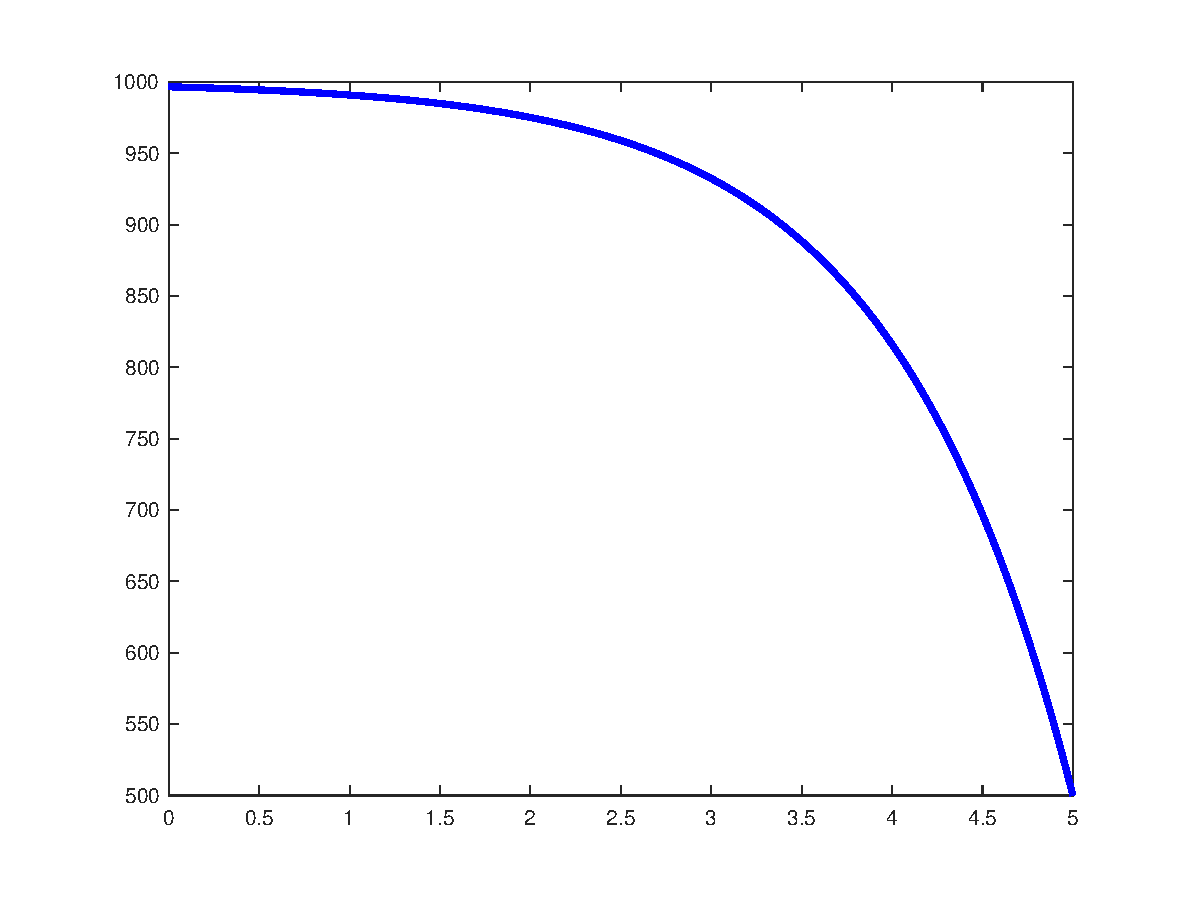
\includegraphics[width=1.5\imagewidth]{Model1-optc.eps}
    \caption{Optimal Control - Model 1}
    \label{fig:model1_optc}
\end{figure}


\begin{figure}[!ht]
    \centering
    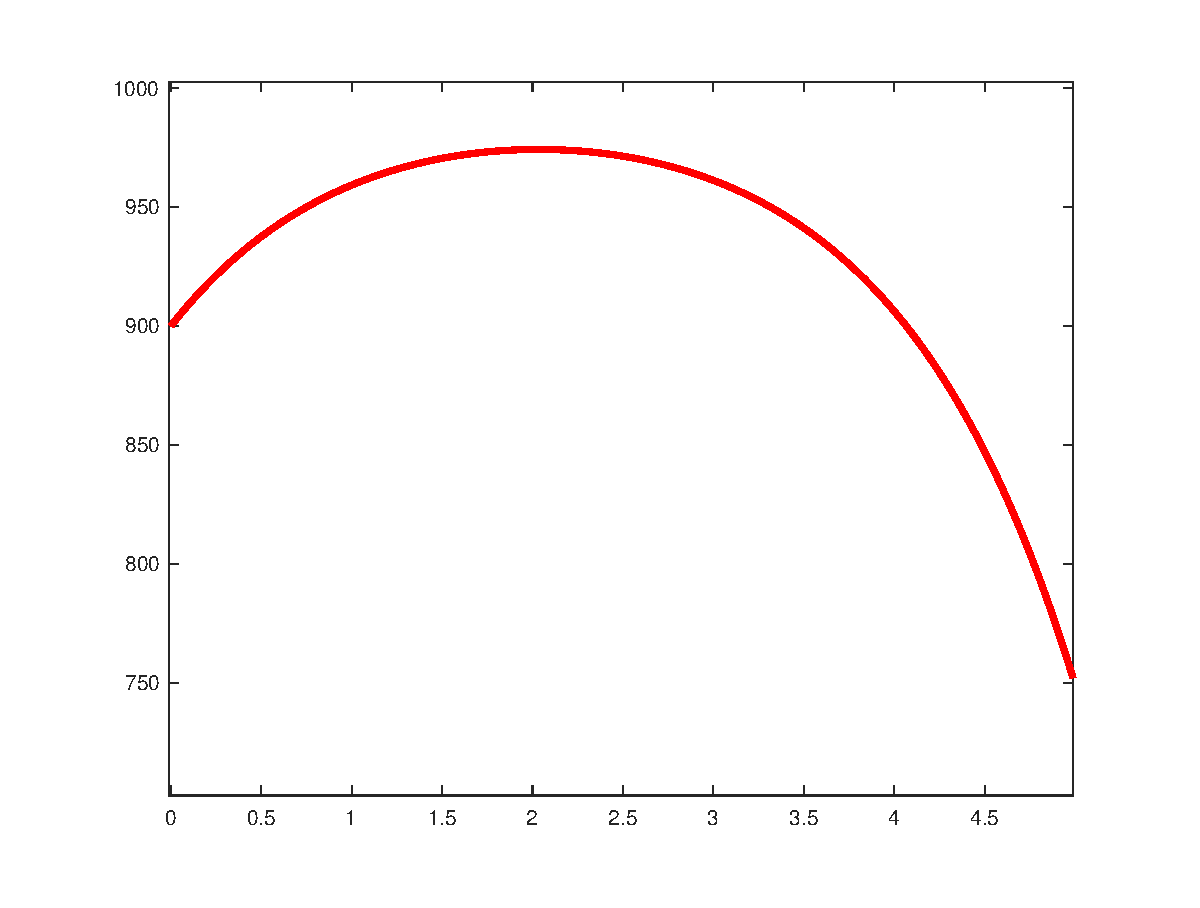
\includegraphics[width=1.5\imagewidth]{Model1-optt.eps}
    \caption{Total Pollution - Model 1}
    \label{fig:model1_optt}
\end{figure}

\newpage

% {\bf Model 1-2(terminal cost):} Our optimization problem is:
% \begin{equation}
%     J(u,T)=\int_{0}^{T}\bigl(-\frac{1}{2}u^2+bu\bigr)dt-Dx(T)\rightarrow \max_{u}\ s.t. \eqref{cd:initial_condition}
% \end{equation}

% Same procedure as \textbf{Model 1-1} item a) to f). The difference between them is there are no boundary conditions on $\psi$ in Model 1-1. But for Model 1-2 is not.

% \begin{equation}
%     \psi(T)=\psi_0 e^{\delta T}=-\frac{d}{dx}Dx(t)\bigg|_{t=T}=-D
% \end{equation}


% Hence:

% \begin{equation}\label{eq1-2:psi0}
%     \psi_0=-De^{-\delta T}
% \end{equation}

% Then,
% \begin{equation}\label{eq1-2:psi}
%     \psi(t)=-De^{\delta (t-T)}
% \end{equation}

% \begin{itemize}
%     \item Substitute Equation \eqref{eq1-2:psi} into Equation \eqref{eq:optc_with_psi}, we can find the optimal control:
%     \begin{equation}
%         u^*(t)=b-De^{\delta (t-T)},\ \text{where}\ b\geq D
%     \end{equation}
%     To maximize the total profit, we should set the maximum control to be greater than $D$.
%     \item Substitute Equation \eqref{eq1-2:psi0} into Equation \eqref{eq:optx_with_psi0}, we get:
%     \begin{equation}\label{eq1-2:optx}
%         x^*(t)=x_0e^{-\delta t}+\frac{b}{\delta}(1-e^{-\delta t})-D\frac{e^{-\delta T}}{2\delta}(e^{\delta t}-e^{-\delta t})
%     \end{equation}

%     The first order derivatives w.r.t $t$ is:

%     \begin{equation}\label{eq1-2:optx_first_order_t}
%         \frac{d x^*(t)}{dt}=b\,{\mathrm{e}}^{-\delta \,t}-\delta \,x_{0}\,{\mathrm{e}}^{-\delta \,t}-\frac{D\,{\mathrm{e}}^{-T\,\delta }\,\left(\delta \,{\mathrm{e}}^{\delta \,t}+\delta \,{\mathrm{e}}^{-\delta \,t}\right)}{2\,\delta }
%     \end{equation}


    
%     % Since the total pollution can not be negative, we need assure $x(t)\geq 0\ \text{for}\ t\in[0,T]$. From the Equation \eqref{eq1-2:optx}, we can find that $t^*$ satisfies $x(t)\geq 0$ for $t\in [0,t^*]$. Therefore for $t\in [0,t^*]$, $x^*(t)$ would following the Equation \eqref{eq1-2:optx} and for $t\in [t^*,T]$, $x^*(t)=0$.




%     {\bf Q1:}
    
%     I think that when function $p(u)$ is satisfies the condition above. Then $f_0(u)=ap(u)$ is satisfies the condition too. Where $a>0$ is a constant.


%     {\bf Q2:}
%     \begin{gather*}
%         J(u,T)=\int_{0}^{T}ap(u)dt-Dx(T) \rightarrow \max_{u}\\
%         \hat{J}(u,T)=\frac{1}{a}J(u,T)=\int_{0}^{T}p(u)dt-\frac{D}{a}x(T) \rightarrow \max_{u}
%     \end{gather*}

%     These two equations are not equivalent? Why just $p(u)$ is linear the assumption is satisfied?

% \end{itemize}


{\bf Model 2:} Our optimization problem is:
\begin{equation}
    J(u,T)=\int_{0}^{T}\ln (u+1)dt-Dx(T)\rightarrow \max_{u}\ s.t. \eqref{cd:initial_condition}
\end{equation}
\begin{enumerate}[a)]
    \item Write down the Hamiltonian Function:
            \begin{equation}\label{eq2:hamiltonian}
                H(x,u,\psi)=\ln (u+1)+\psi (u-\delta x)
            \end{equation}
    \item It's first order partial derivatives w.r.t $u$ is:
            \begin{equation}
                \frac{\partial }{\partial u}H(x,u,\psi)=\frac{1}{u+1}+\psi
            \end{equation}
             According to the first order extreme condition:
             \begin{equation}\label{eq2:optc_with_psi}
                u^*(t)=-\frac{1}{\psi}-1
             \end{equation}
             And $\frac{\partial^2 }{\partial u^2}H(x,u,\psi)\big|_{u=u^*}<0$, we can conclude that the Hamiltonian $H$ is concave w.r.t $u$.
    \item We substituete \eqref{eq2:optc_with_psi} into \eqref{eq2:hamiltonian} to get the maximal Hamiltonian Function:
             \begin{equation}
                \mathcal{H}(x, \psi)=H(x,u^*,\psi)=-\ln(-\psi)-(1+\psi)-\psi\delta x
             \end{equation}
    \item The canonical form is written as:
             \begin{equation}\label{eq2:canonical_form}
                 \begin{dcases}
                    \dot{x}= \frac{\partial }{\partial \psi}H(x,u,\psi)\bigg|_{u=u^*}=-\frac{1}{\psi}-1-\delta x\\
                    \dot{\psi}=-\frac{\partial }{\partial x}H(x,u,\psi)\bigg|_{u=u^*}=\delta \psi(t)
                \end{dcases}
             \end{equation}
    \item From D.E.S \eqref{eq2:canonical_form}, it's not hard to find:
             \begin{equation}\label{eq2:psi_with_psi0}
                 \psi(t)=\psi_0 e^{\delta t}
             \end{equation}
    \item According to D.E.S \eqref{eq2:canonical_form} and Equation \eqref{eq2:psi_with_psi0}, we can find the optimal trajectory:
             \begin{equation}\label{eq2:optx_with_psi0}
                 x^*(t)={\mathrm{e}}^{-\delta \,t}\,\left(x_{0}+\frac{1}{\delta }\right)-{\mathrm{e}}^{-\delta \,t}\,\left(\frac{t}{\psi _{0}}+\frac{{\mathrm{e}}^{\delta \,t}}{\delta }\right)
             \end{equation}
    \item There is boundary condition on $\psi$:
    \begin{equation}
        \psi(T)=\psi_0 e^{\delta T}=-\frac{d}{dx}Dx(t)\bigg|_{t=T}=-D
    \end{equation}

    Hence:

    \begin{equation}\label{eq2:psi0}
        \psi_0=-De^{-\delta T}
    \end{equation}

    Then,
    \begin{equation}\label{eq2:psi}
        \psi(t)=-De^{\delta (t-T)}
    \end{equation}

    \item Substitute Equation \eqref{eq2:psi} into Equation \eqref{eq2:optc_with_psi}, we can find the optimal control:
    \begin{equation}
        u^*(t)=\frac{e^{\delta(T-t)}}{D}-1,\ \text{where}\ \frac{e^{\delta T}}{D}-1\leq b,\ \text{and}\ 0\leq D\leq1
    \end{equation}

    We need to assure $u^*(t)\in [0,b]\ \text{for}\ t\in[0,T]$, so condition $\frac{e^{\delta T}}{D}-1\leq b\ \text{and}\ 0\leq D\leq 1$ is necessary,

    \item Substitute Equation \eqref{eq2:psi0} into Equation \eqref{eq2:optx_with_psi0}, we get:
    \begin{equation}\label{eq2:optx}
        x^*(t)={\mathrm{e}}^{-\delta \,t}\,\left(x_{0}+\frac{1}{\delta }\right)-{\mathrm{e}}^{-\delta \,t}\,\left(-\frac{te^{\delta T}}{D}+\frac{{\mathrm{e}}^{\delta \,t}}{\delta }\right)
    \end{equation}


    \item  Find the first order derivative w.r.t $t$:
    \begin{equation}\label{eq2:optx_d}
        \frac{dx^*(t)}{dt}=-\frac{{\mathrm{e}}^{-\delta \,t}\,\left(D-{\mathrm{e}}^{T\,\delta }+D\,\delta \,x_{0}+\delta \,t\,{\mathrm{e}}^{T\,\delta }\right)}{D}
    \end{equation}

    Under the condition below: 

    \begin{equation}\label{conditions:model2}
        \begin{split}
            \frac{e^{\delta T}}{D}-1\leq b\\
            D\leq 1\\
            D+D\,\delta \,x_{0}<{\mathrm{e}}^{T\,\delta }\\
            \text{all parameters are large than 0}
        \end{split}
    \end{equation}

    We can find the stationary point:

    \begin{equation}\label{eq2:t^*}
        t^*=-\frac{{\mathrm{e}}^{-T\,\delta }\,\left(D-{\mathrm{e}}^{T\,\delta }+D\,\delta \,x_{0}\right)}{\delta }
    \end{equation}

    Obviously, $\frac{dx^*(t)}{dt}<0\ \text{for}\ t\in [0,t^*)$ and $\frac{dx^*(t)}{dt}\geq 0\ \text{for}\ t\in [t^*,T]$.
    
    So, $x^*(t)$ reachs maximal value at $t=t^*$.

    \item Check the second sufficient condition for the existence of extreme values. Find the second order derivative w.r.t $t$: 

    \begin{equation}\label{eq2:second_order_t}
        \frac{d^2x^*(t)}{dt^2}=\frac{\delta \,{\mathrm{e}}^{-\delta \,t}\,\left(D-2\,{\mathrm{e}}^{T\,\delta }+D\,\delta \,x_{0}+\delta \,t\,{\mathrm{e}}^{T\,\delta }\right)}{D}
    \end{equation}

    Substitute $t^*$ into Equation \eqref{eq2:second_order_t}:
    
    \begin{equation}
        \frac{d^2x^*(t)}{dt^2}\bigg|_{t=t^*}=-\frac{\delta \,{\mathrm{e}}^{T\,\delta }\,{\mathrm{e}}^{D\,{\mathrm{e}}^{-T\,\delta }+D\,\delta \,x_{0}\,{\mathrm{e}}^{-T\,\delta }-1}}{D}<0
    \end{equation}

    So, $x^*(t)$ reachs maximal value at $t=t^*$.

    \item Assure $x^*(t)\geq 0,\ \text{for}\ t\in[0,T]$.
    
    % Substitute $t^*$ into Equation \eqref{eq2:optx}, we can easily find:
    % \begin{equation}\label{eq2:x^*_t*}
    %     x^*(t^*)=\frac{b\,\sqrt{2\,b\,{\mathrm{e}}^{T\,\delta }-D-2\,\delta \,x_{0}\,{\mathrm{e}}^{T\,\delta }}-2\,\sqrt{D}\,b+D^{3/2}\,{\mathrm{e}}^{-T\,\delta }+2\,\sqrt{D}\,\delta \,x_{0}}{\delta \,\sqrt{2\,b\,{\mathrm{e}}^{T\,\delta }-D-2\,\delta \,x_{0}\,{\mathrm{e}}^{T\,\delta }}}
    % \end{equation}

    % Under the Conditions \eqref{conditions:model2}, we can make sure:

    % \begin{equation*}
    %     \delta \,\sqrt{2\,b\,{\mathrm{e}}^{T\,\delta }-D-2\,\delta \,x_{0}\,{\mathrm{e}}^{T\,\delta }}>0
    % \end{equation*}

    Since the function $x^*(t)$ is concave for $t\in[0,T]$. To assure $x^*(t)\geq 0$ for all $t\in [0,T]$. We only need to make sure the boundary points large than $0$, w.r.t $x_0\geq 0\ \text{and}\ x^*(T)\geq 0$.

    Substitute $t=T$ into Equation \eqref{eq2:optx}, we can get the terminal value of $x^*$ w.r.t $x^*(T)$:

    \begin{equation}
        x^*(T)=\frac{T\,\delta -D+D\,{\mathrm{e}}^{-T\,\delta }+D\,\delta \,x_{0}\,{\mathrm{e}}^{-T\,\delta }}{D\,\delta }
    \end{equation}

    Obviously, $D\delta>0$, so we need add the condition:

    \begin{equation}\label{conditionForxT:model2}
        T\,\delta -D+D\,{\mathrm{e}}^{-T\,\delta }+D\,\delta \,x_{0}\,{\mathrm{e}}^{-T\,\delta }\geq 0
    \end{equation}

    \item If we need to assure that the terminal value of pollutions is less than the initial value, we can abtain the conditon by the following Expression:
    
    \begin{equation}\label{conditionForx_Tandx_0:model2}
        x^*(T)<x_0
    \end{equation}

    From the Expression \eqref{conditionForx_Tandx_0:model2}, we can get :

    \begin{equation}\label{conditionForx_Tandx_02:model2}
        \frac{T\,\delta -D+D\,{\mathrm{e}}^{-T\,\delta }+D\,\delta \,x_{0}\,{\mathrm{e}}^{-T\,\delta }}{D\,\delta }<x_0
    \end{equation}

\end{enumerate}

{\bf Summarize of Model 2:}

After the above steps, we got some Conditions \eqref{conditions:model2}, \eqref{conditionForxT:model2} and \eqref{conditionForx_Tandx_02:model2}, combine them, I get:

\begin{equation}\label{conditions:finally_model2}
    \begin{split}
        \frac{e^{\delta T}}{D}-1\leq b\\
        D\leq 1\\
        D+D\,\delta \,x_{0}<{\mathrm{e}}^{T\,\delta }\\
        T\,\delta -D+D\,{\mathrm{e}}^{-T\,\delta }+D\,\delta \,x_{0}\,{\mathrm{e}}^{-T\,\delta }\geq 0\\
        T\delta+D(e^{-T\delta}-1)(1+\delta x_0)<0\\
        % T\,\delta -D+D\,{\mathrm{e}}^{-T\,\delta }+D\,\delta \,x_{0}\,{\mathrm{e}}^{-T\,\delta }-D\delta x_0<0\\
        \text{all parameters are large than 0}
    \end{split}
\end{equation}

The following is also those conditions but genereted by MATLAB. The condition above is equivalent to the condition below.

\begin{equation}
\left(\begin{array}{ccccccccccc} D+D\,\delta \,x_{0}<{\mathrm{e}}^{T\,\delta } \\ 0\leq T\,\delta -D+D\,{\mathrm{e}}^{-T\,\delta }+D\,\delta \,x_{0}\,{\mathrm{e}}^{-T\,\delta } \\ \frac{{\mathrm{e}}^{T\,\delta }}{D}-1\leq b \\ 0<D \\ D\leq 1 \\ 0<T \\ 0<b \\ 0<\delta  \\ 0<t \\ 0<x_{0} \\ \frac{T\,\delta -D+D\,{\mathrm{e}}^{-T\,\delta }+D\,\delta \,x_{0}\,{\mathrm{e}}^{-T\,\delta }}{D\,\delta }<x_{0} \end{array}\right)
\end{equation}

Now, I choose some parameters which satisfy the conditions \eqref{conditions:finally_model2}. When T is too large, it is difficult to select other parameters that meet the above conditions. So, I choose a small one that $T=5$. Corresponding, we need to change unit of our time from  day to year. $x_0=100, b=200, D=0.9, \delta=1 $.

The Figure of optimal control and total pollution as shown in Figure \ref{fig:model2_optc} and Figure \ref{fig:model2_optt}:


\begin{figure}[!ht]
    \centering
    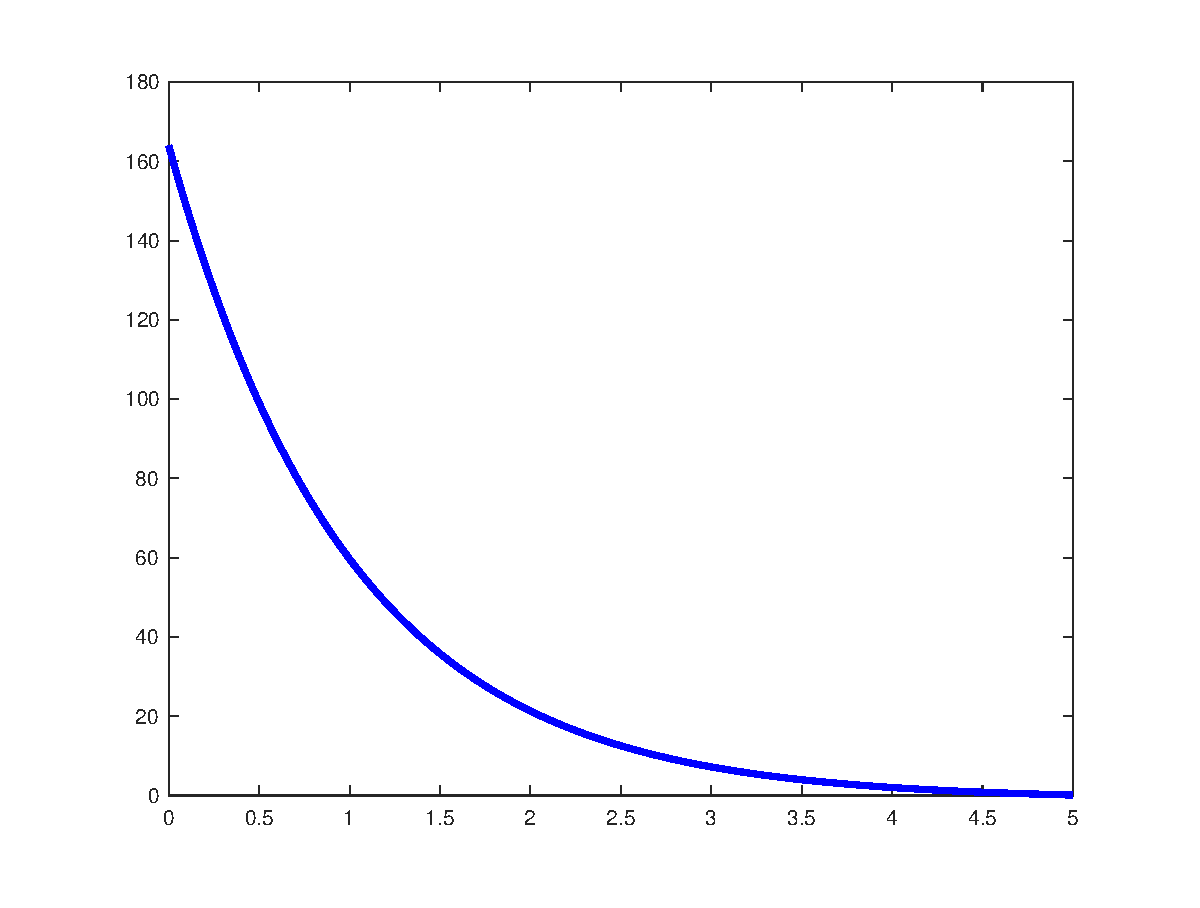
\includegraphics[width=1.5\imagewidth]{Model2-optc.eps}
    \caption{Optimal Control - Model 2}
    \label{fig:model2_optc}
\end{figure}


\begin{figure}[!ht]
    \centering
    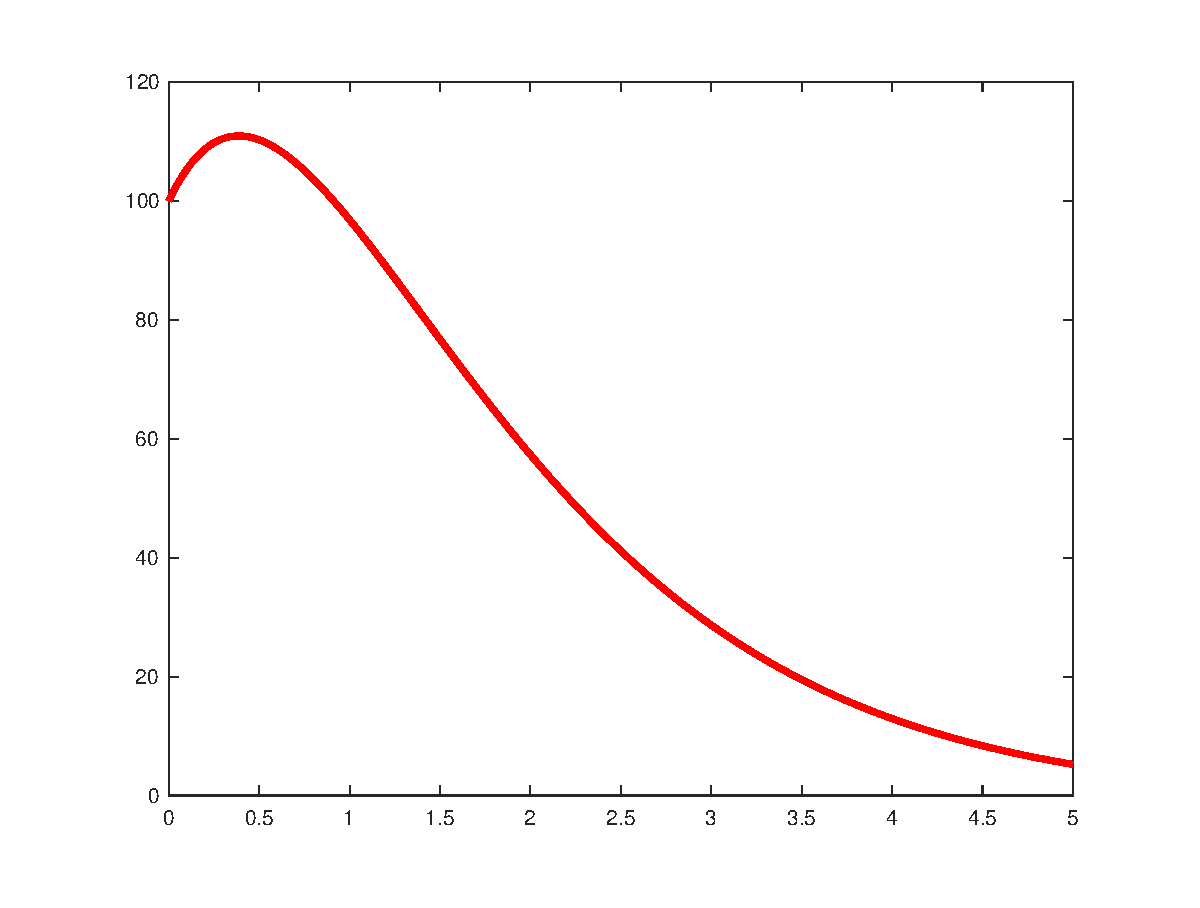
\includegraphics[width=1.5\imagewidth]{Model2-optt.eps}
    \caption{Total Pollution - Model 2}
    \label{fig:model2_optt}
\end{figure}


{\bf Summary:}

From the first order derivative of $x^*(t)$ w.r.t $t$, Equation \eqref{eq1:optx_d} and Equation \eqref{eq2:optx_d}, we can get some conditions which is necessary since we need to assure $x^*(t)\geq 0$ for all $t\in[0,T]\ \text{and}\ x(T)\le x_0$. By comparing these conditions, it's easily to find that the conditions of logarithmic form utility function is simpler be find than quadratic form utility function. The reason is the different location of $t$ marked in the following Equation. The previous one is exponential function, and another is linear function. So, the Expressions of Conditions of Model 2 is simpler than Model 1.

\begin{gather*}
    \begin{split}
        {\bf Model\ 1:}&\frac{dx^*(t)}{dt}=-{\mathrm{e}}^{-\delta \,\left(T+t\right)}\,\left(\frac{D}{2}-b\,{\mathrm{e}}^{T\,\delta }+\frac{D\,{\mathrm{e}}^{2\,\delta \,\textcolor{red}{t}}}{2}+\delta \,x_{0}\,{\mathrm{e}}^{T\,\delta }\right)\\
        {\bf Model\ 2:}&\frac{dx^*(t)}{dt}=-\frac{{\mathrm{e}}^{-\delta \,t}\,\left(D-{\mathrm{e}}^{T\,\delta }+D\,\delta \,x_{0}+\delta \,\textcolor{red}{t}\,{\mathrm{e}}^{T\,\delta }\right)}{D}
    \end{split}
\end{gather*}

The utility function can influence the results. The optimal control is dependent to the utilify function. And the optimal trajectory is dependent to the optimal control. Then, for different utility functions, the company can use different controls to achieve the goal of maximizing profits.

\end{document}

